\section{Supplementary Material}

\subsection{Qualitative Results}

\subsubsection{MNIST-ROT}

% \begin{figure}[h]
% \centering
% \includegraphics[width=\textwidth]{img/mnist_rot_raw_im.png}
% \caption{t-SNE visualization of raw MNIST-ROT images}
% \end{figure}

% \begin{figure}[h]
% \centering
% 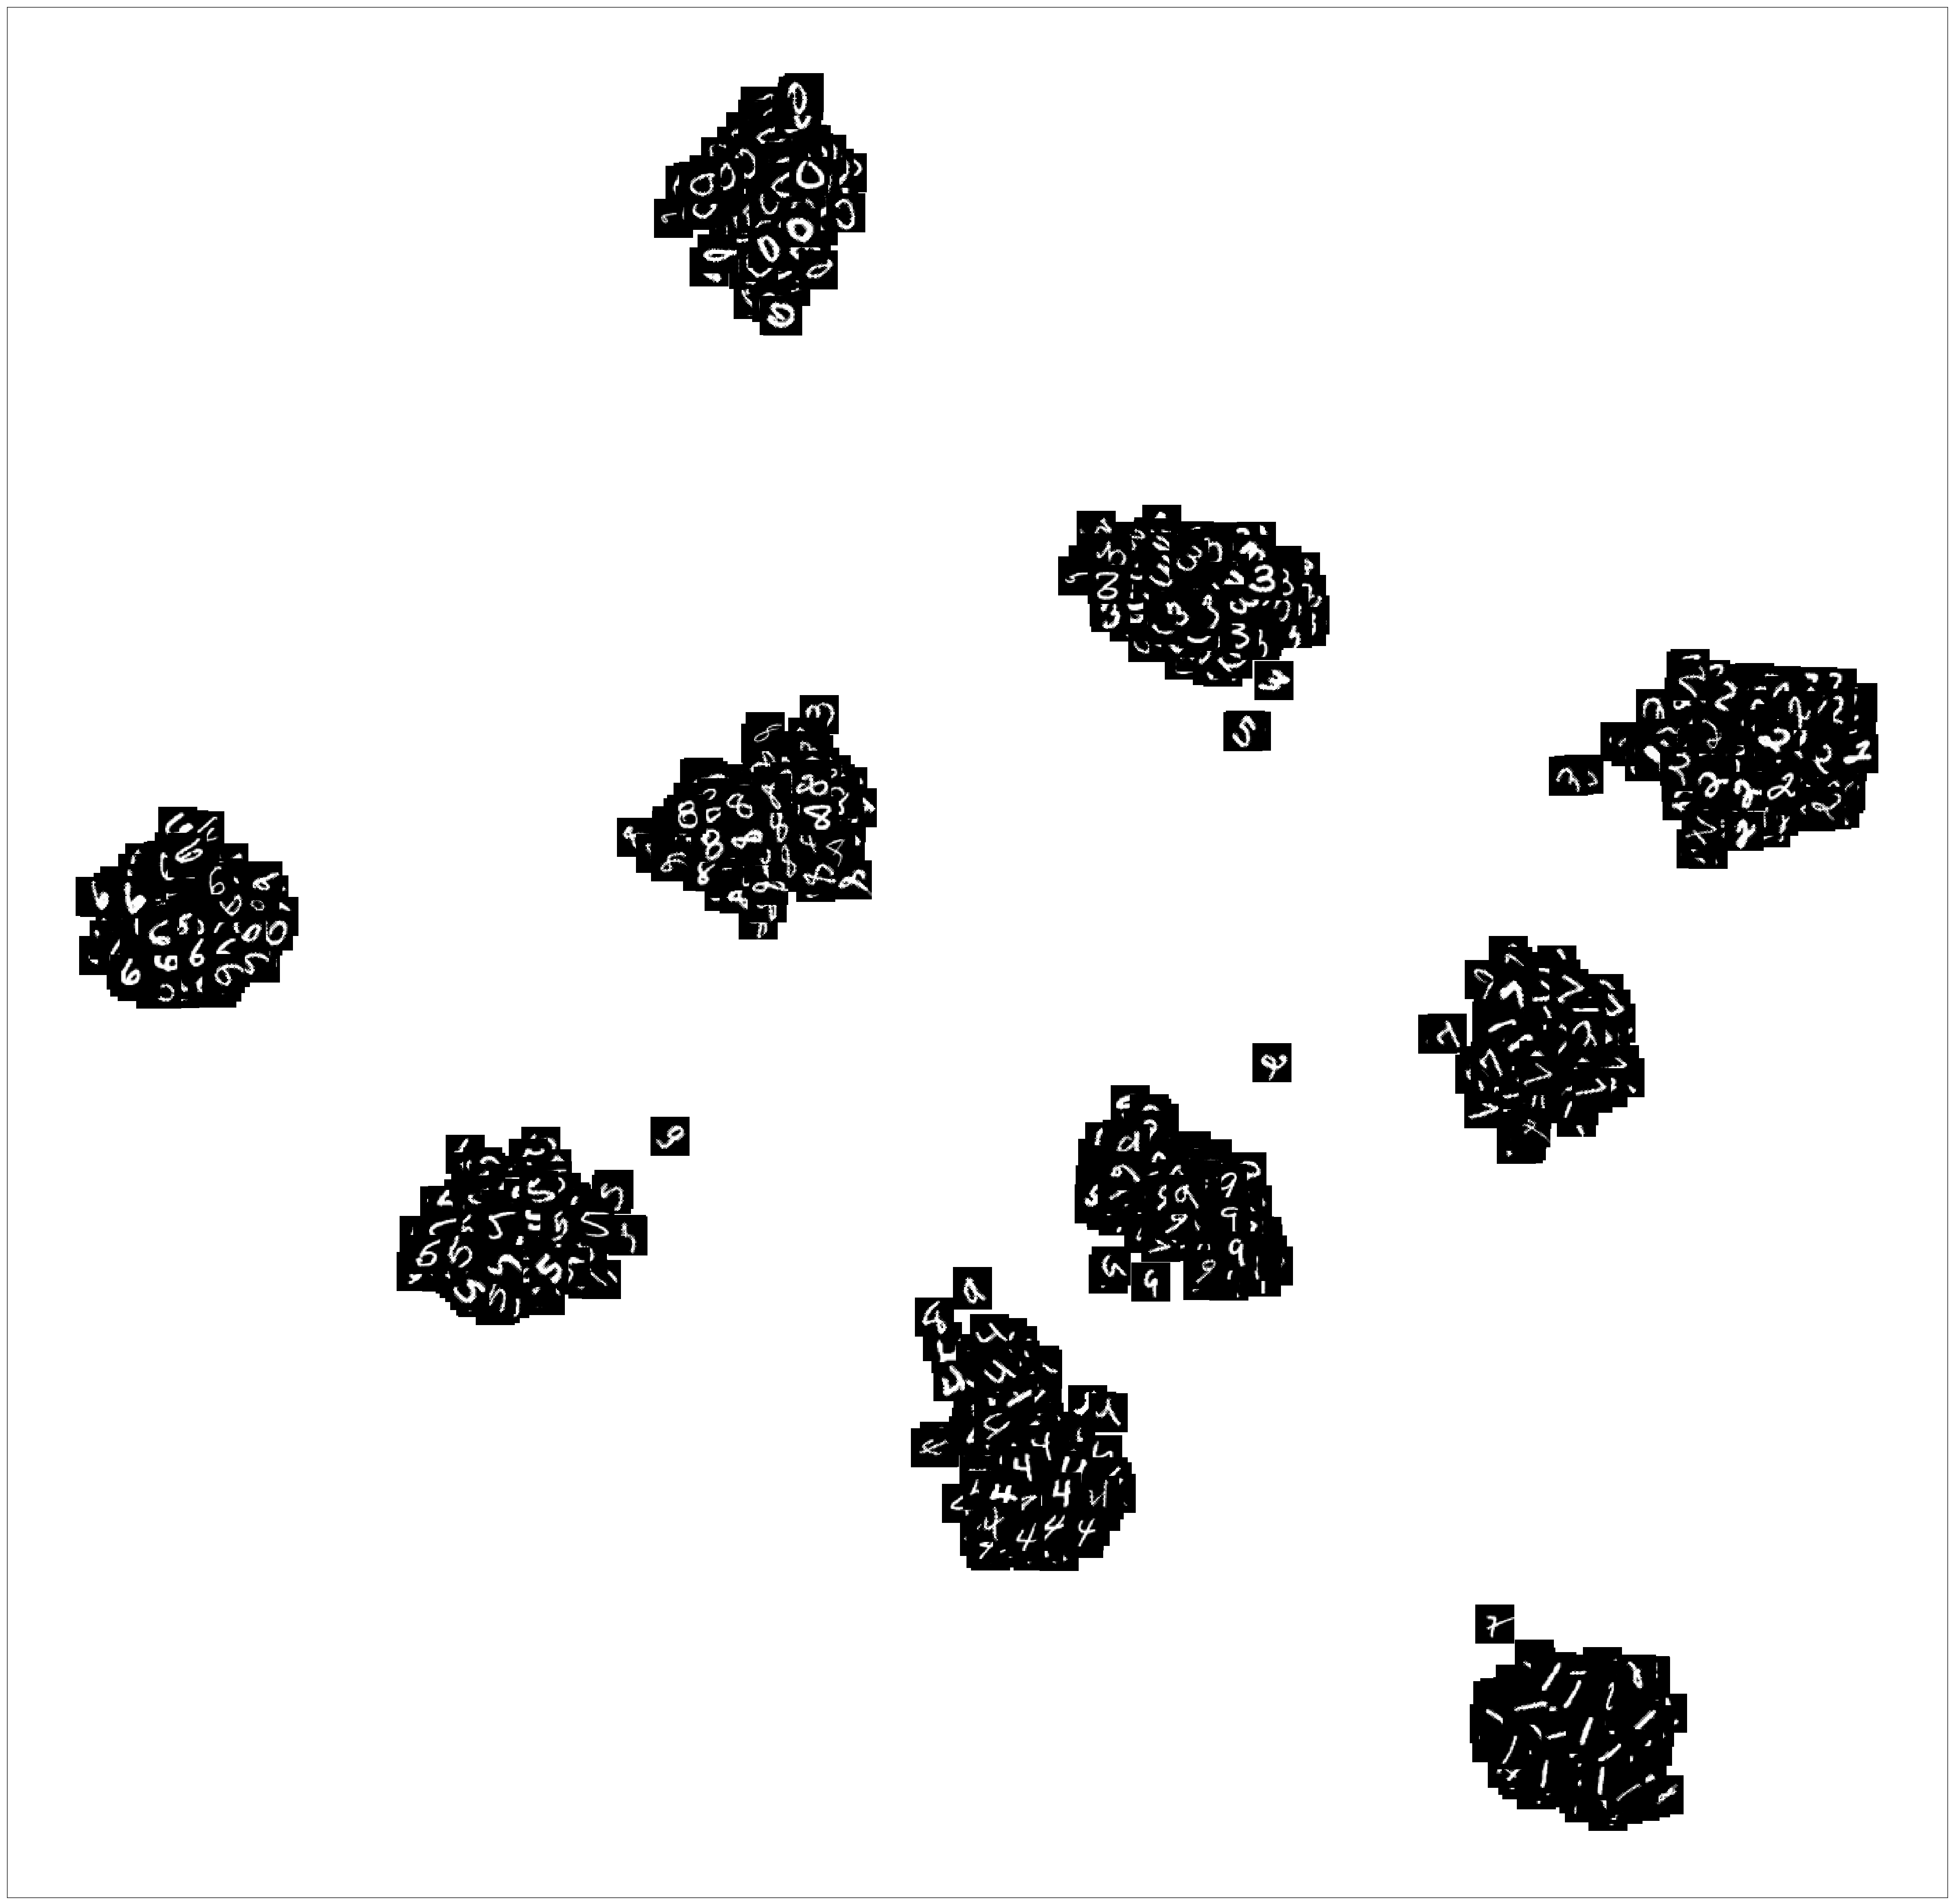
\includegraphics[width=\textwidth]{img/mnist_rot_e1_im.png}
% \caption{t-SNE visualization of MNIST-ROT $e_1$ embedding. Model trained on $\Theta = \{-45, -22.5, 0, 22.5, 45\}$.}
% \end{figure}

\begin{figure}[h]
\centering
\begin{subfigure}{0.45\textwidth}
\centering
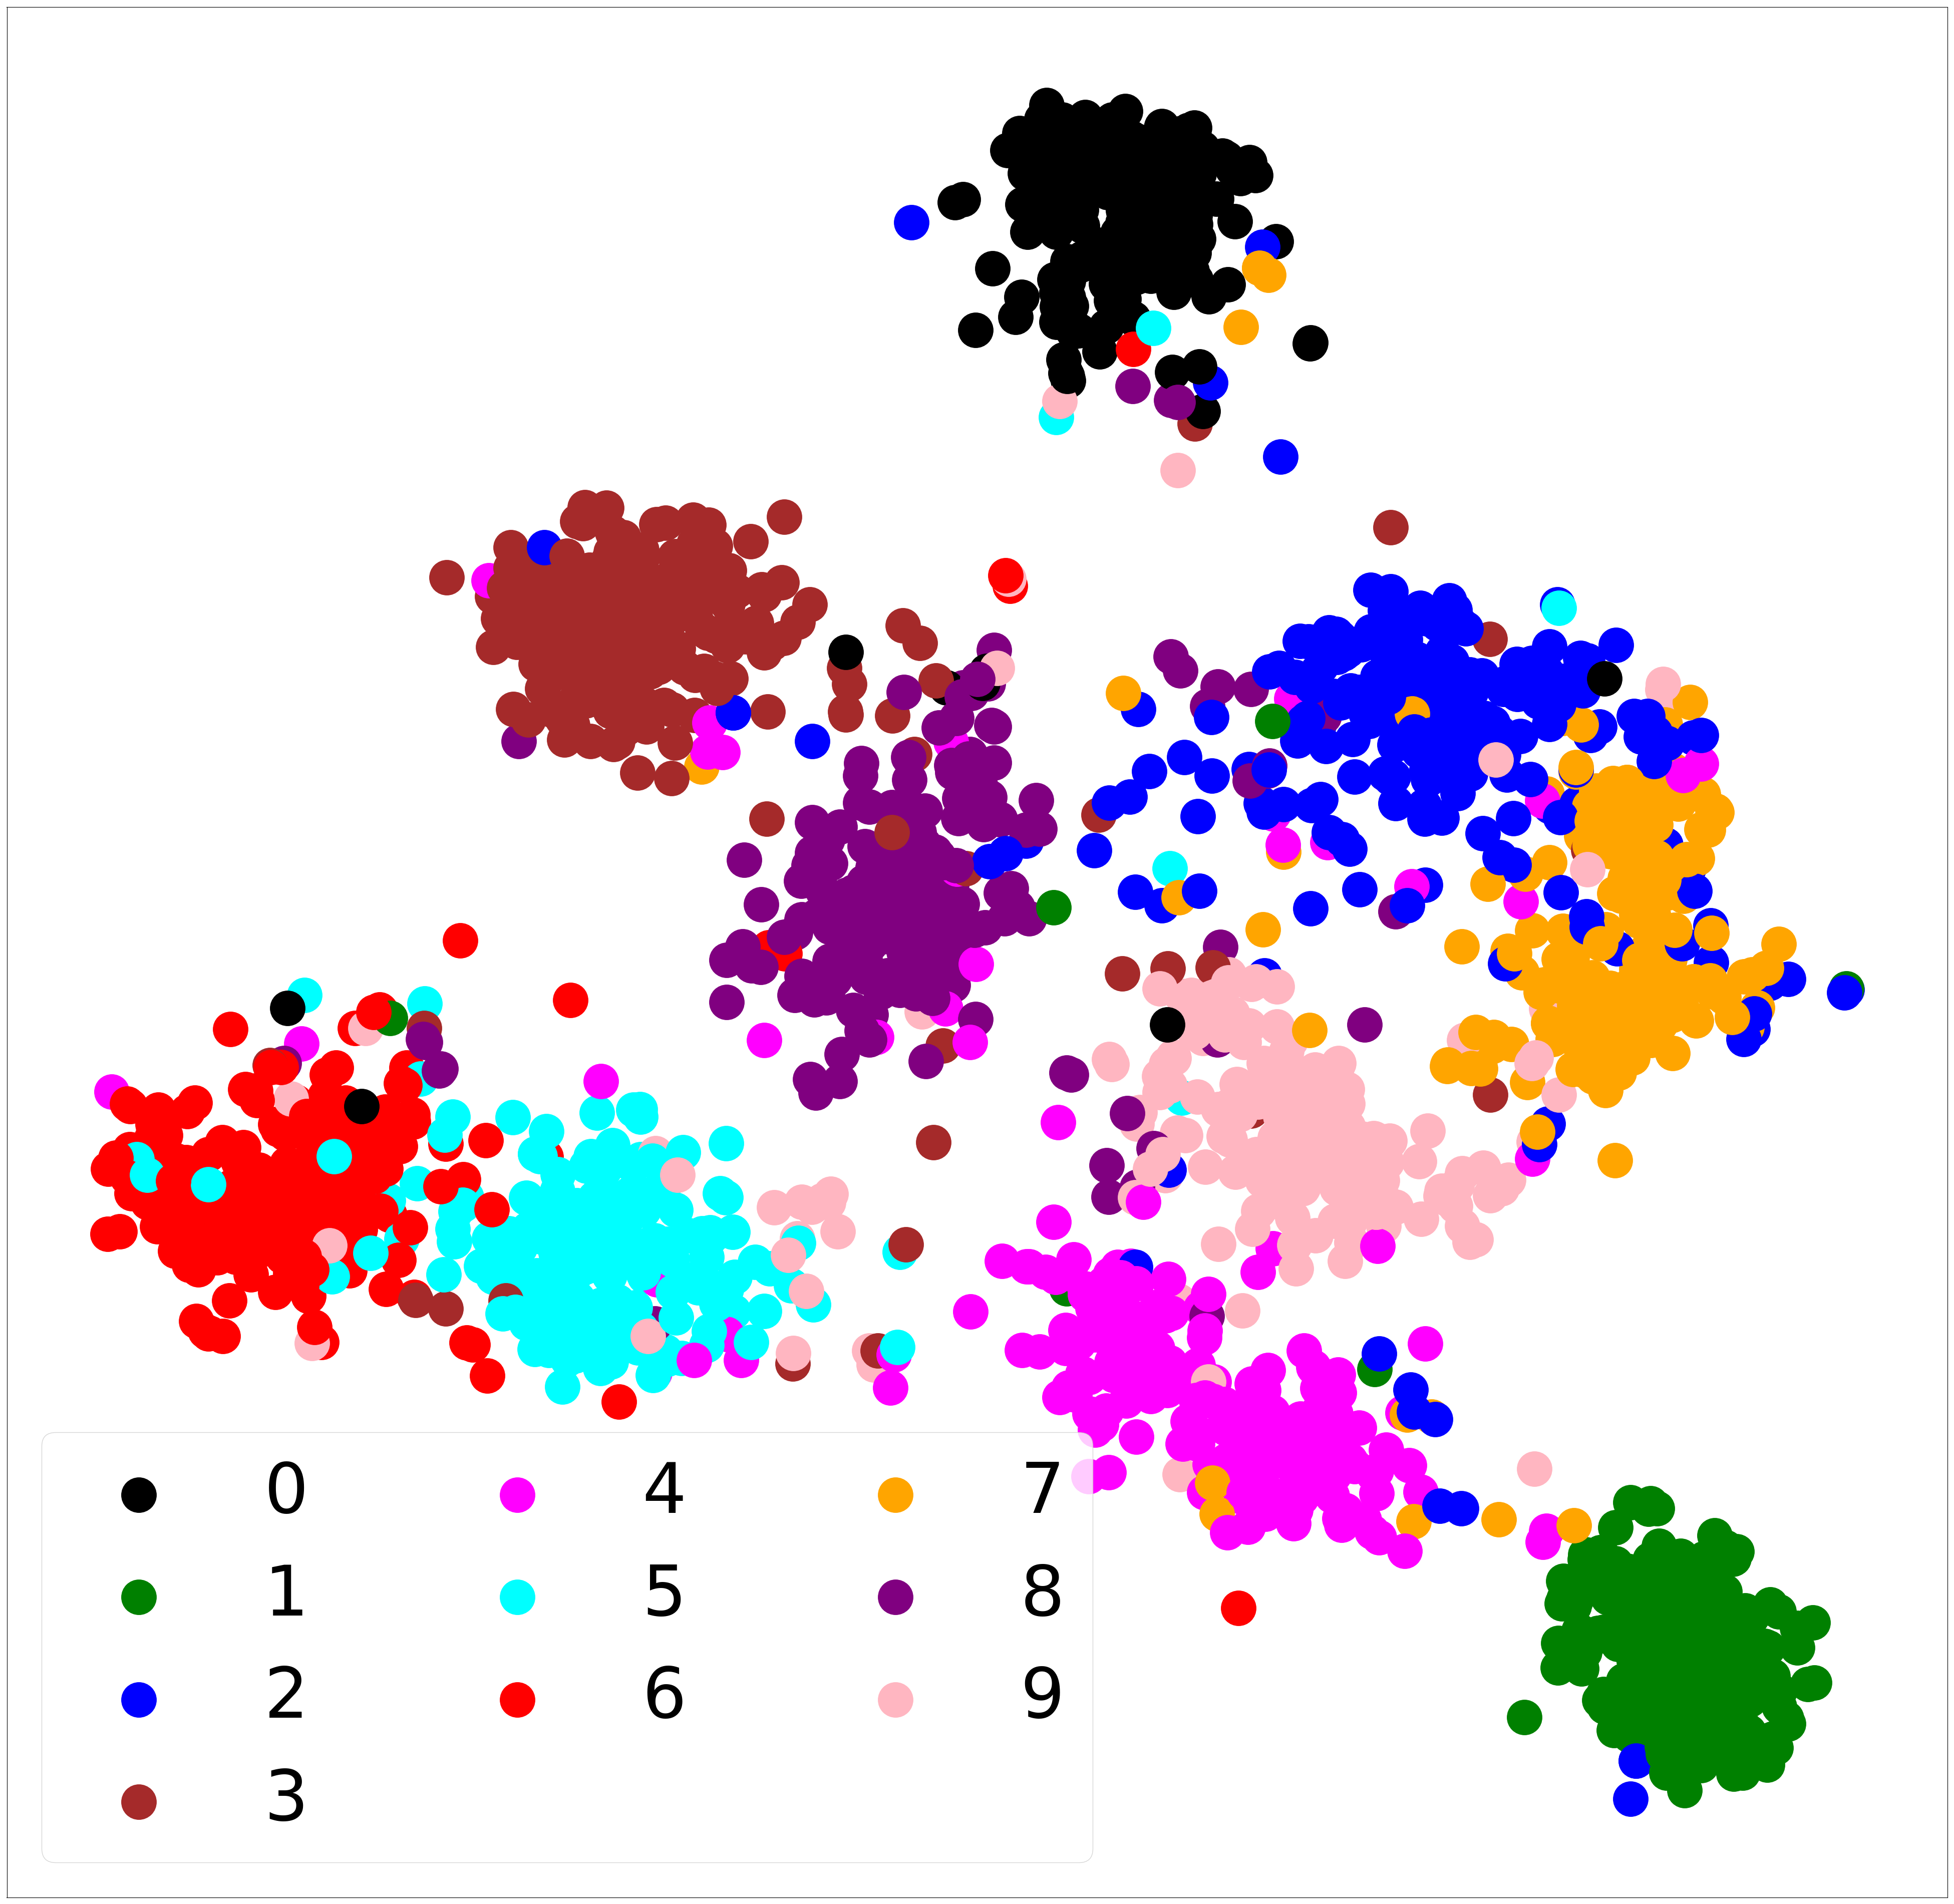
\includegraphics[width=\textwidth]{img/supp_mnist_rot_e1_label_55.png}
\end{subfigure}
\hfill
\begin{subfigure}{0.45\textwidth}
\centering
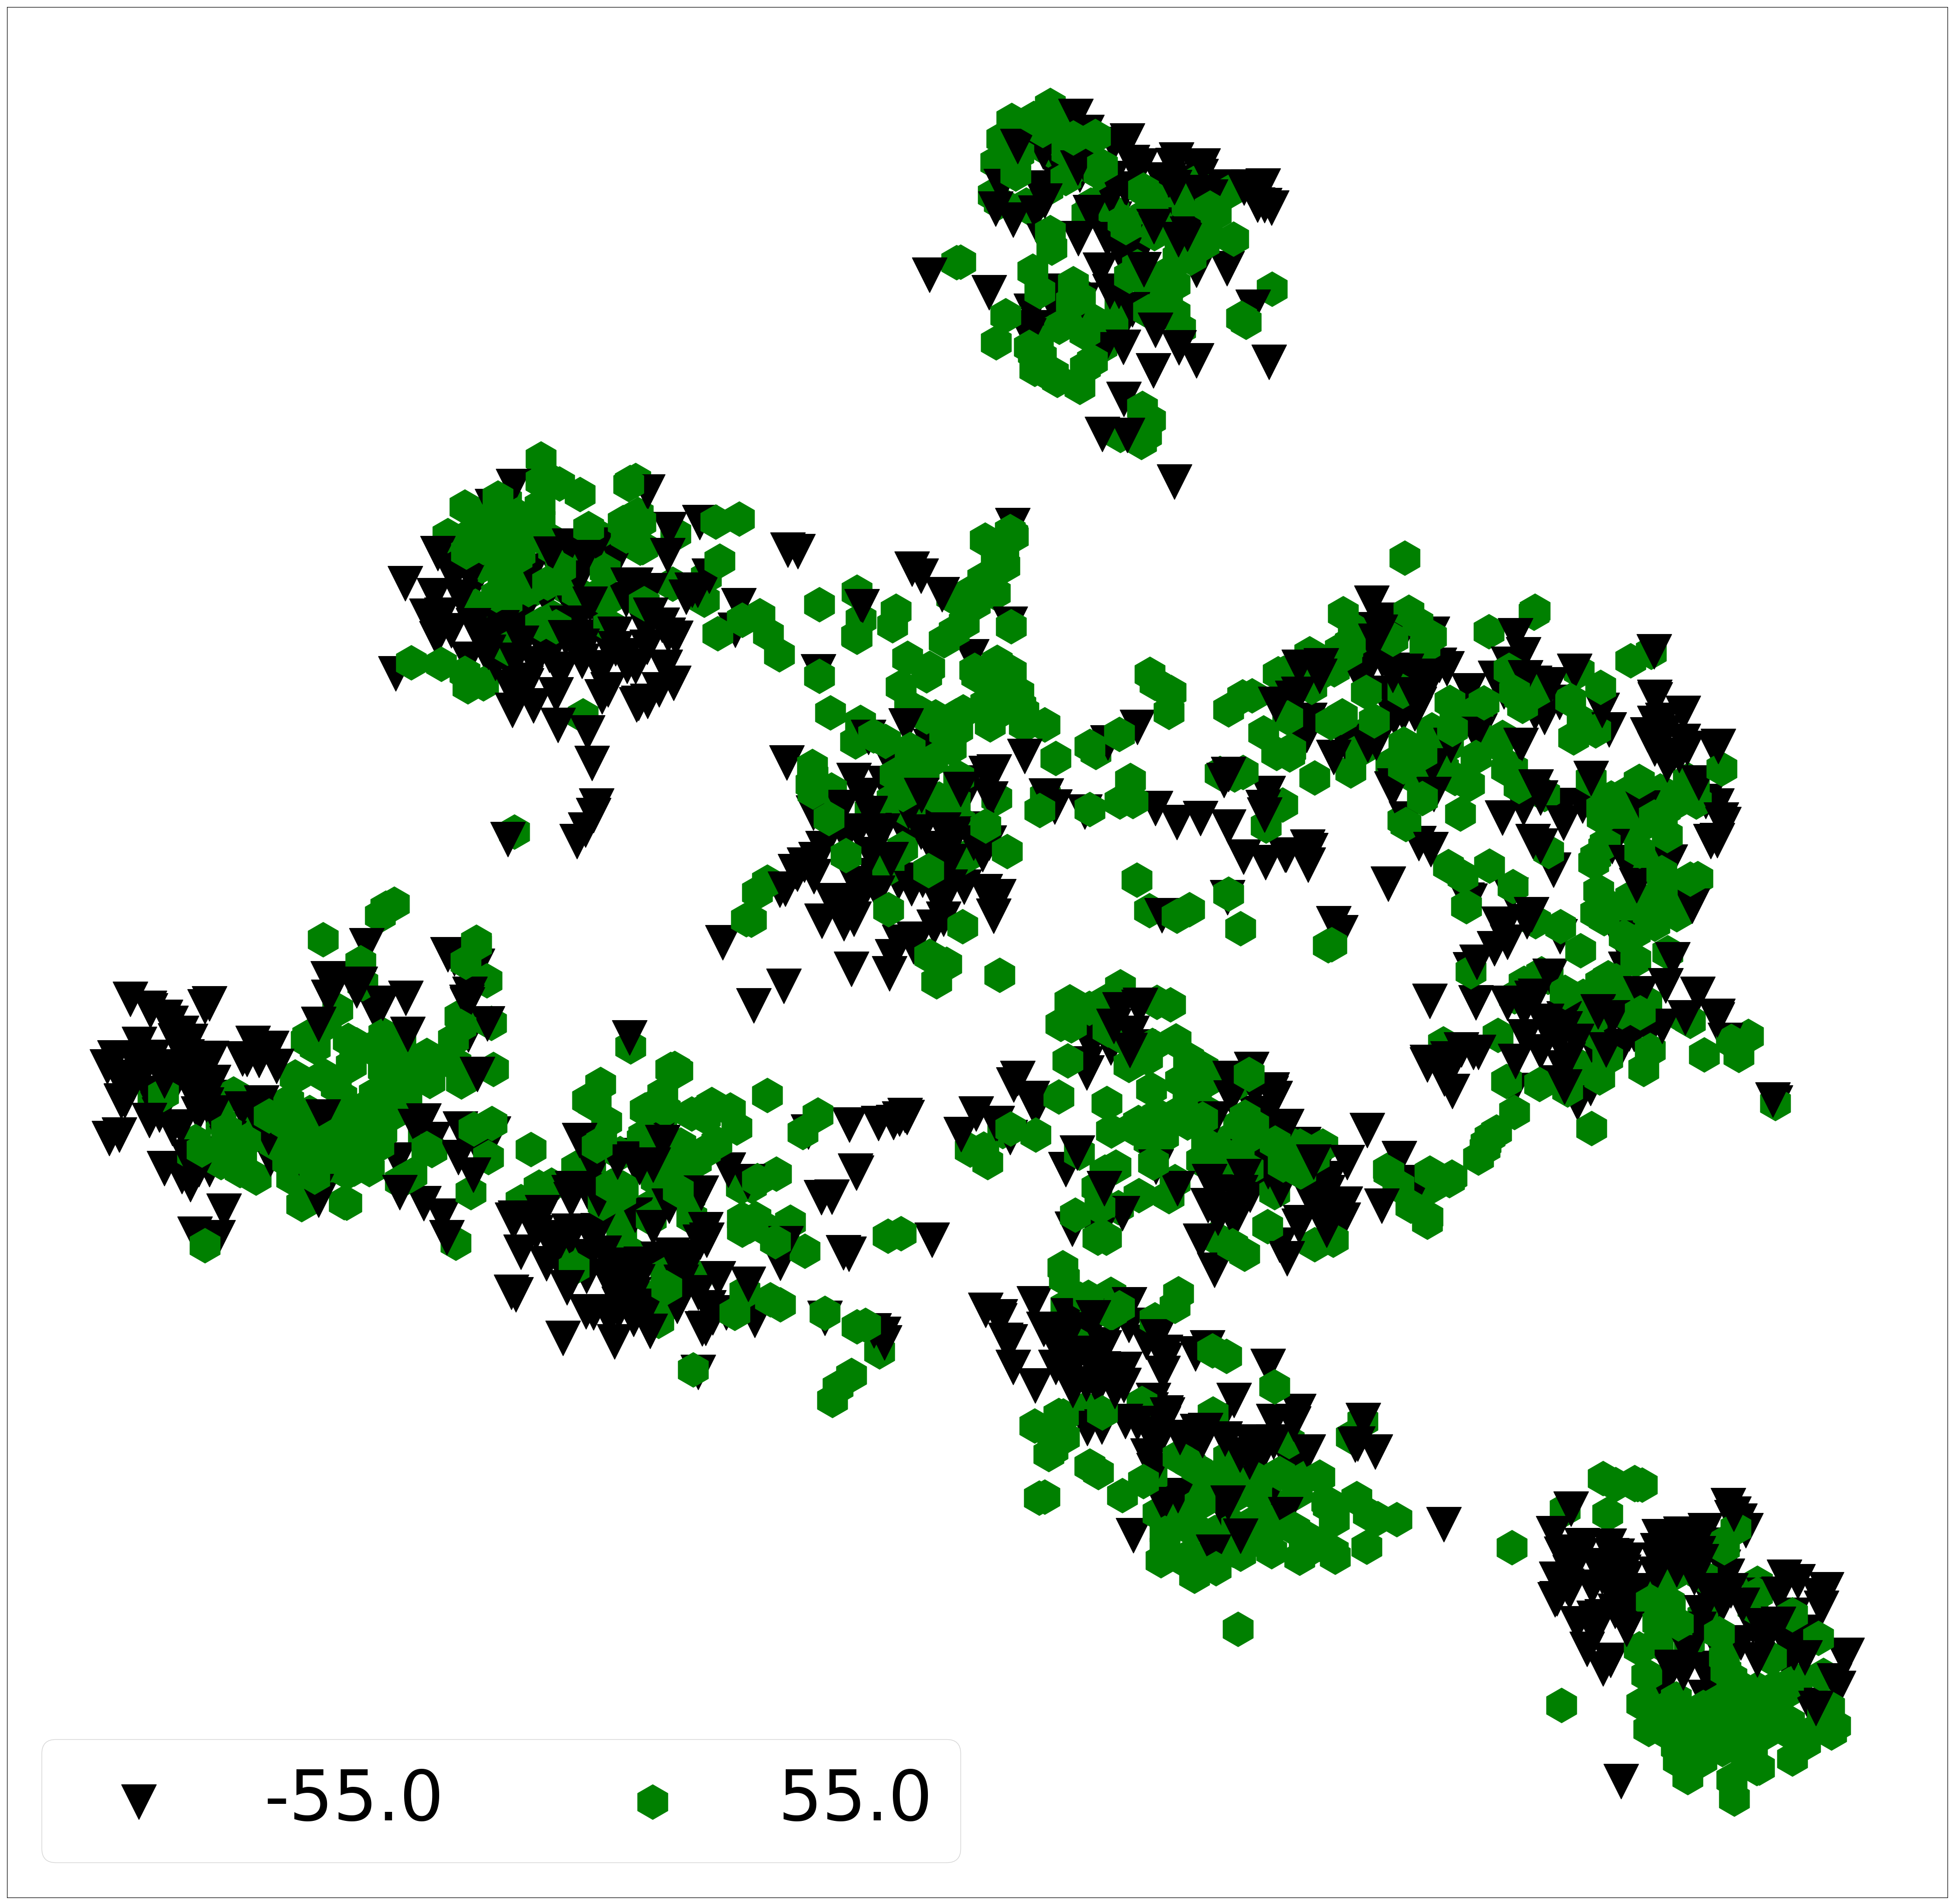
\includegraphics[width=\textwidth]{img/supp_mnist_rot_e1_label_55_z.png}
\end{subfigure}
\caption{\label{fig:e1_55}t-SNE visualization of MNIST-ROT $e_1$ embedding for the proposed Unsupervised Adversarial Invariance model. Model trained on $\Theta = \{0, \pm22.5, \pm45\}$. Visualization generated for $\Theta = \{\pm55\}$. Embedding $e_1$, which is used to predict $y$, shows no clustering by the rotation angle.}
\end{figure}

\begin{figure}[h]
\centering
\begin{subfigure}{0.45\textwidth}
\centering
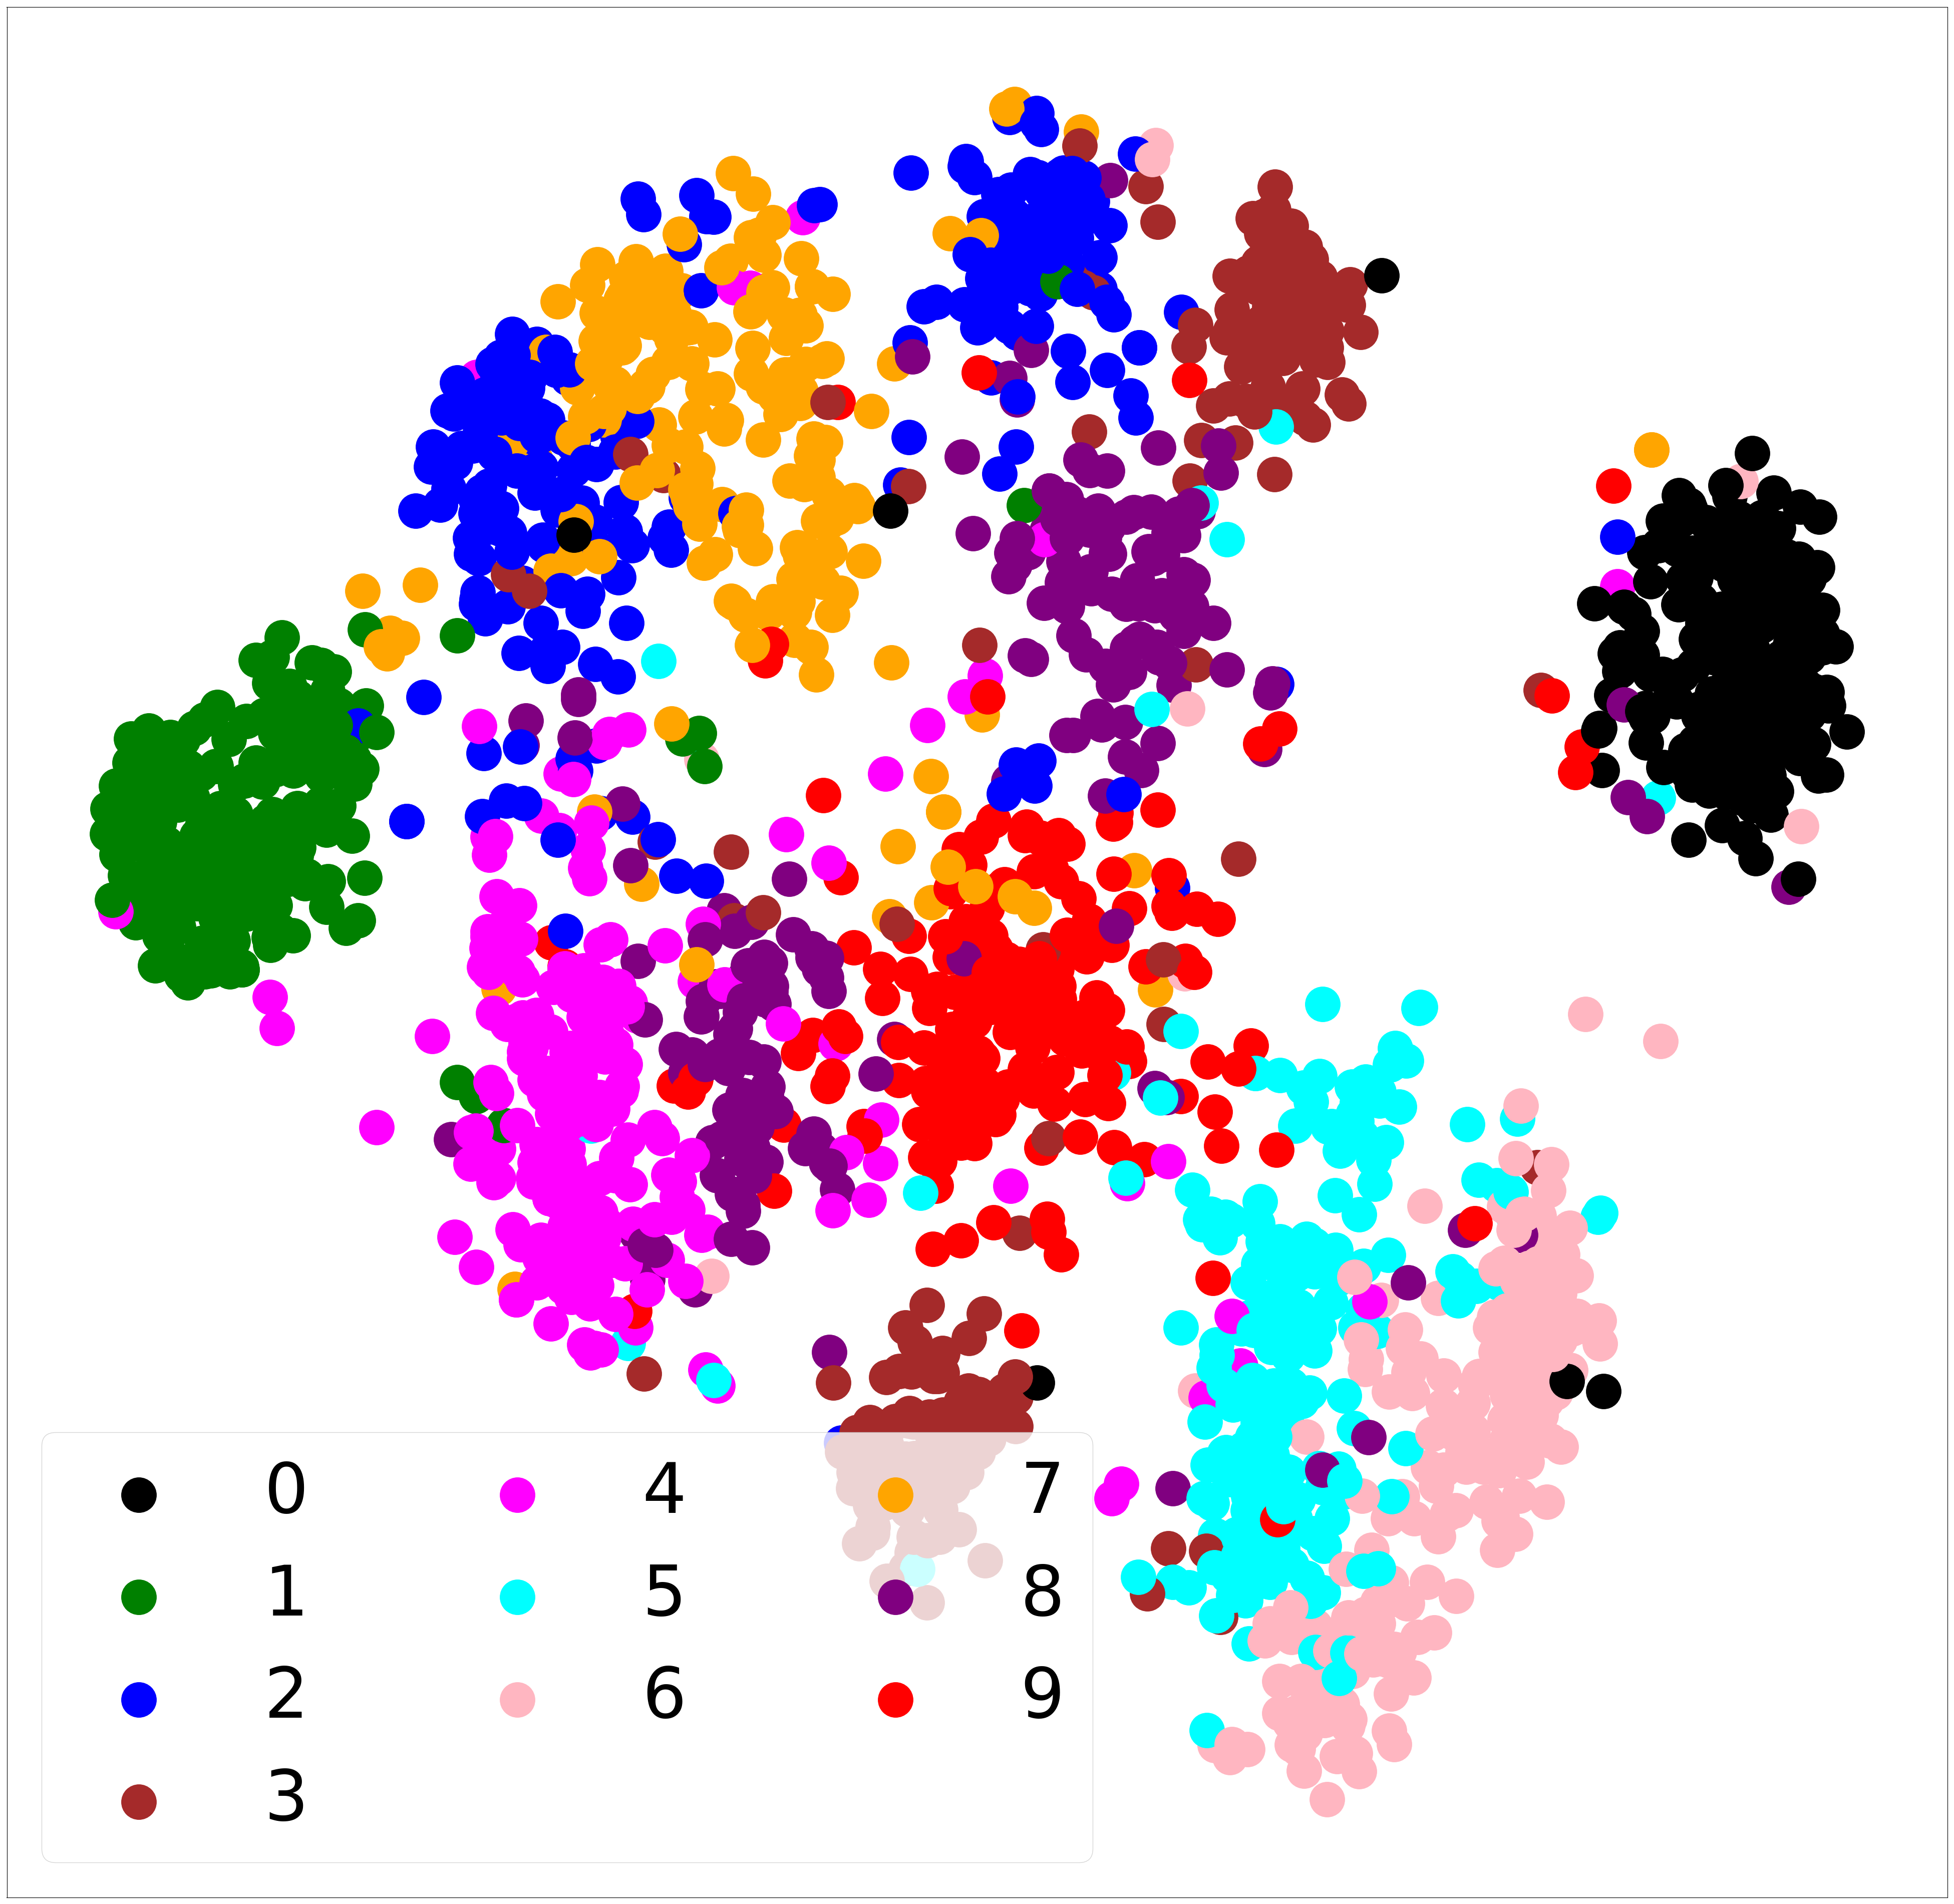
\includegraphics[width=\textwidth]{img/supp_mnist_rot_e1_label_55_b0.png}
\end{subfigure}
\hfill
\begin{subfigure}{0.45\textwidth}
\centering
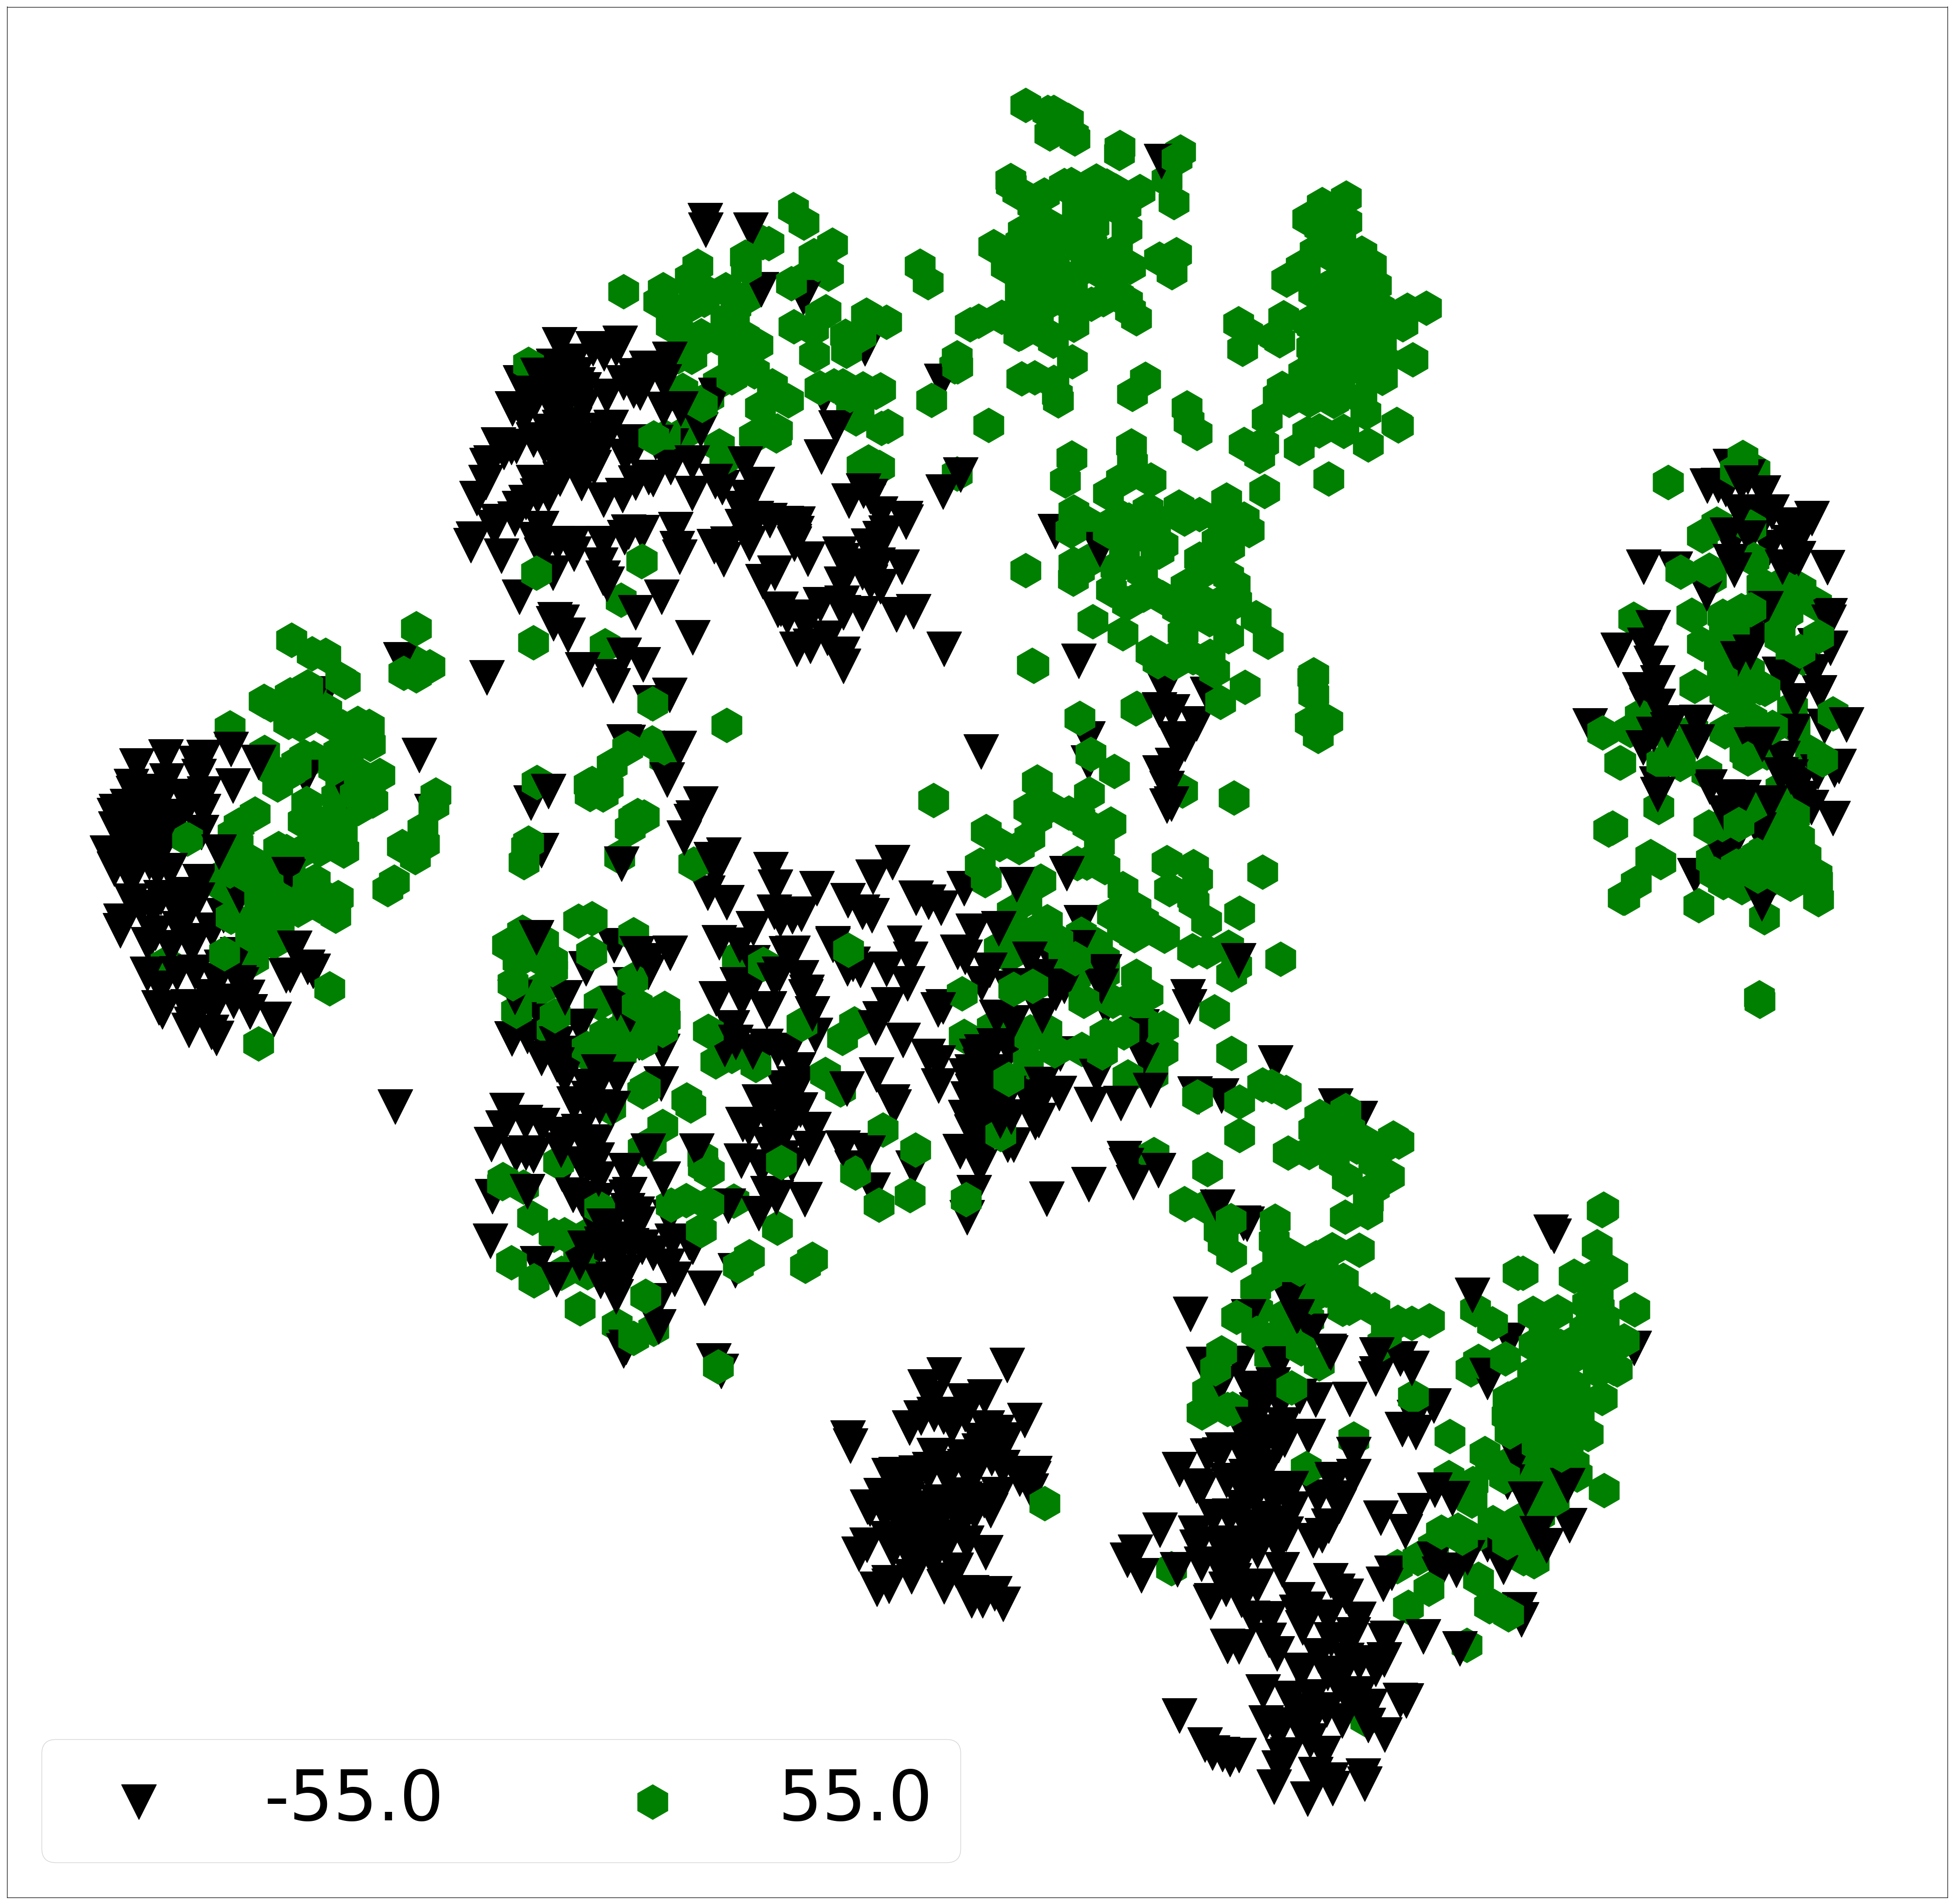
\includegraphics[width=\textwidth]{img/supp_mnist_rot_e1_label_55_z_b0.png}
\end{subfigure}
\caption{\label{fig:e1_55_b0}t-SNE visualization of MNIST-ROT $e_1$ embedding for baseline model $B_0$, which only models $x \rightarrow h \rightarrow y$. Model trained on $\Theta = \{0, \pm22.5, \pm45\}$. Visualization generated for $\Theta = \{\pm55\}$. Embedding $e_1$, which is used to predict $y$, shows clustering by the rotation angle, with encodings of some digit classes forming multiple clusters corresponding to rotation angles.}
\end{figure}

\clearpage

\begin{figure}[h]
\centering
\includegraphics[width=0.875\textwidth]{img/supp_mnist_recon_e1_new.png}
\caption{Reconstruction from $e_1$}
\end{figure}

\begin{figure}[h]
\centering
\includegraphics[width=0.875\textwidth]{img/supp_mnist_recon_e2_new.png}
\caption{Reconstruction from $e_2$}
\end{figure}

\begin{figure}[h]
\centering
\includegraphics[width=0.875\textwidth]{img/supp_mnist_recon_e1e2_new.png}
\caption{Reconstruction from $e = [e_1 \ e_2]$}
\end{figure}

\clearpage

\subsection{Extended Yale-B}

\begin{figure}[h]
\centering
\begin{subfigure}{0.65\textwidth}
\centering
\includegraphics[width=\textwidth]{img/supp_yaleb_raw_im.png}
\end{subfigure}
\hfill
\begin{subfigure}{0.65\textwidth}
\centering
\includegraphics[width=\textwidth]{img/supp_yaleb_raw_label.png}
\end{subfigure}
\caption{\label{fig:eyb_raw}t-SNE visualization of raw Extended Yale B images. Raw data is clustered by lighting.}
\end{figure}

\begin{figure}[h]
\centering
\begin{subfigure}{0.75\textwidth}
\centering
\includegraphics[width=\textwidth]{img/supp_yaleb_e1_im.png}
\end{subfigure}
\hfill
\begin{subfigure}{0.75\textwidth}
\centering
\includegraphics[width=\textwidth]{img/supp_yaleb_e1_label.png}
\end{subfigure}
\caption{\label{fig:eyb_raw}t-SNE visualization of $e_1$ for Extended Yale B. Markers are numbers denoting subject-ID. There are 38 subjects in this dataset. $e_1$ is clustered by subject identity. $e_1$ encoding of images of the same subject but with different lighting conditions get clustered together.}
\end{figure}

\begin{figure}[h]
\centering
\begin{subfigure}{0.75\textwidth}
\centering
\includegraphics[width=\textwidth]{img/supp_yaleb_e2_im.png}
\end{subfigure}
\hfill
\begin{subfigure}{0.75\textwidth}
\centering
\includegraphics[width=\textwidth]{img/supp_yaleb_e2_label.png}
\end{subfigure}
\caption{\label{fig:eyb_raw}t-SNE visualization of $e_2$ for Extended Yale B. $e_2$ is clustered by lighting condition.}
\end{figure}

\clearpage
\begin{figure}[h]
\centering
\includegraphics[width=0.8\textwidth]{img/supp_yaleb_recon_e1_new.png}
\captionsetup{aboveskip=-5pt}
\caption{Reconstruction from $e_1$}
\end{figure}
\vspace{-20pt}
\begin{figure}[h]
\centering
\includegraphics[width=0.8\textwidth]{img/supp_yaleb_recon_e2_new.png}
\captionsetup{aboveskip=-5pt}
\caption{Reconstruction from $e_2$}
\end{figure}
\vspace{-20pt}
\begin{figure}[h]
\centering
\includegraphics[width=0.8\textwidth]{img/supp_yaleb_recon_e1e2_new.png}
\captionsetup{aboveskip=-5pt}
\caption{Reconstruction from $e = [e_1 \ e_2]$}
\end{figure}
\vspace{-20pt}

\clearpage
\subsubsection{Chairs}

\begin{figure}[h]
\centering
\includegraphics[width=0.875\textwidth]{img/supp_chairs_recon_e1_new.png}
\caption{Reconstruction from $e_1$}
\end{figure}

\begin{figure}[h]
\centering
\includegraphics[width=0.875\textwidth]{img/supp_chairs_recon_e2_new.png}
\caption{Reconstruction from $e_2$}
\end{figure}

\clearpage
\subsection{Quantitative Results}

Quantitative results of predicting nuisance factors $z$ from $e_1$, which is expected to contain only factors of variation of $x$ relevant to predicting $y$ and no $z$, and $e_2$, which is expected to contain $z$, are presented in Table~\ref{tab:e1e2}. These nuisance factors are lighting conditions in case of Extended Yale-B, rotation angle used to synthesize images in MNIST-ROT, and yaw angle of Chairs images. The results quantitatively validate the desired information separation expected in our framework.

\makegapedcells
\begin{table}[h]
\centering
\caption{Accuracy of predicting $z$ from $e_1$ and $e_2$}
\label{tab:e1e2}
\begin{tabular}{ c ?{1.5pt} c ?{1.5pt} c }
  \hbline
  \textbf{Dataset} & \textbf{Accuracy of predicting $z$ from $e_1$} & \textbf{Accuracy of predicting $z$ from $e_2$} \\
  \hbline
  Extended Yale-B & 0.24 & 0.89 \\
  MNIST-ROT & 0.34 & 0.77 \\
  Chairs & 0.34 & 0.73 \\
  \hbline
\end{tabular}
\end{table}